\section{Noise Generation}

When evaluating image processing algorithms, it is important to see how they perform under various levels of noise.


\begin{figure}[ht]
\centering
	\subfigure[Original image]{
	
\includegraphics[width=0.45\linewidth]{question2/toy}
	}
\end{figure}

\begin{figure}[ht]
\centering
	\subfigure[Image with Gaussian Noise; $\sigma^2$=0.01]{
	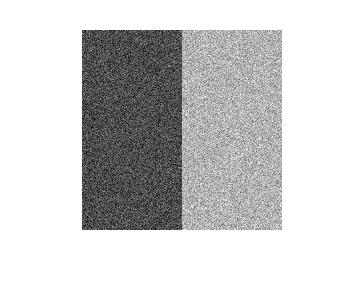
\includegraphics[width=0.45\linewidth]{question2/gauss}
	}
	\subfigure[Histogram of Gaussian Noise Image]{
	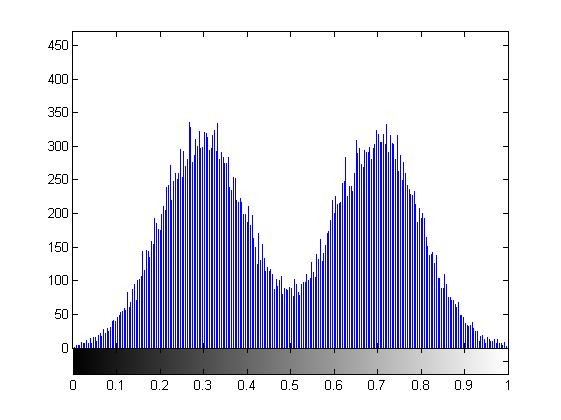
\includegraphics[width=0.45\linewidth]{question2/gauss_hist}
	}
	\subfigure[Image with Speckle Noise; $\sigma^2$=0.04]{
	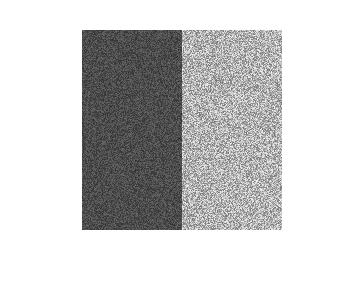
\includegraphics[width=0.45\linewidth]{question2/speckle}
	}
	\subfigure[Histogram of Speckle Noise Image]{
	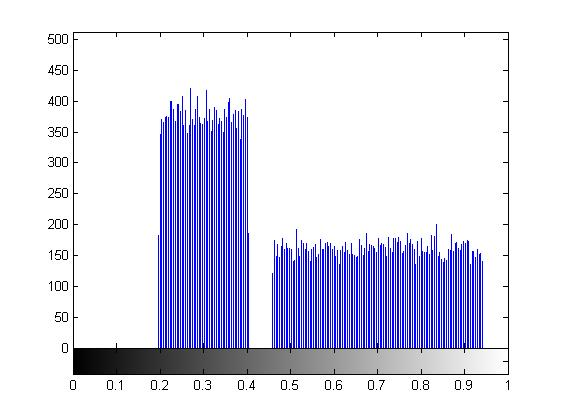
\includegraphics[width=0.45\linewidth]{question2/speckle_hist}
	}
	\subfigure[Image with Salt and Pepper Noise; $\rho$=0.05]{
	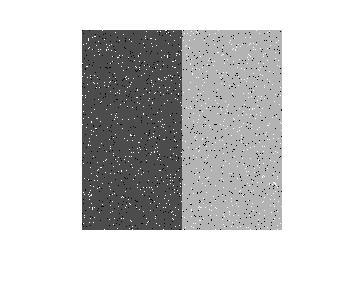
\includegraphics[width=0.45\linewidth]{question2/salt}
	}
	\subfigure[Histogram of Salt and Pepper Image]{
	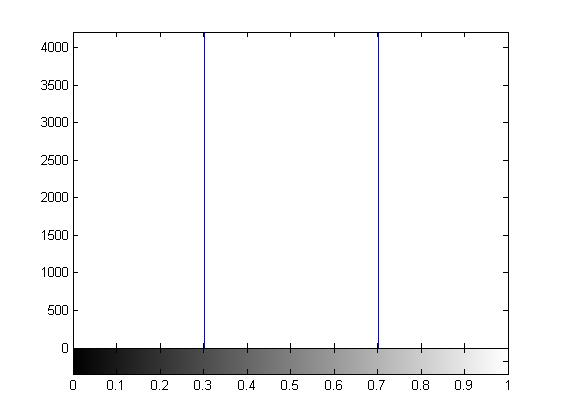
\includegraphics[width=0.45\linewidth]{question2/salt_hist}
	}
	\caption{Toy image with Gaussian, Salt and Pepper, and Speckle Noise}
	\label{fig:noiseGeneration.toy}
\end{figure}
 

\subsection{Discussion questions}

\subsubsection{ Describe each of the histograms in the context of the corresponding noise models. Why do they appear
that way?}
In the Gaussian histogram, image intensities are grouped in Gaussian distributions centred around the two intensity values of the original image. It appears the way it is because as additive noise, all that is being done is the Gaussian distribution is added to the image. Speckled noise, which is multiplicative, appears to be a flat distribution centred around the original intensities. There is more variance around the higher original intensity value, which is due to the multiplicative nature of speckle noise.

\subsubsection{Are there visual differences between the noise contaminated images? What are they? Why}
There are some visual differences. The Gaussian has a lot more extra bright or extra dark pixels, while speckled has more that are more off by a smaller intensity. This is because the Gaussian is additive noise, and the speckled is multiplicative.

\subsubsection{In the speckle noise case, what is the underlying distribution used? Can you tell from the histogram?
How?}
The underlying distribution is uniform. You can tell from the histogram because the intensities are distributed roughly evenly (i.e. same number of pixels). 

\subsubsection{In the speckle noise case, you will notice that the peaks of the histogram are no longer of the same
height as they were in the original image. Also, the spread around each of the peaks is also different
from each other. Why? Hint: Noise is multiplicative}
Since the noise is multiplicative, it is proportional to the local grey level in the image. i.e. there will be a wider spread of values around higher grey levels, as we can see with the right-most spread having a higher variance.
